\documentclass[11pt,a4paper]{article}
\usepackage[english]{babel}
\usepackage[utf8]{inputenc}
\usepackage{verbatim}
\usepackage{amssymb}
\usepackage{graphicx}

\title{BW4T - Refactoring}

\date{\today}

\begin{document}

\maketitle

\section{Hoe het nu is}
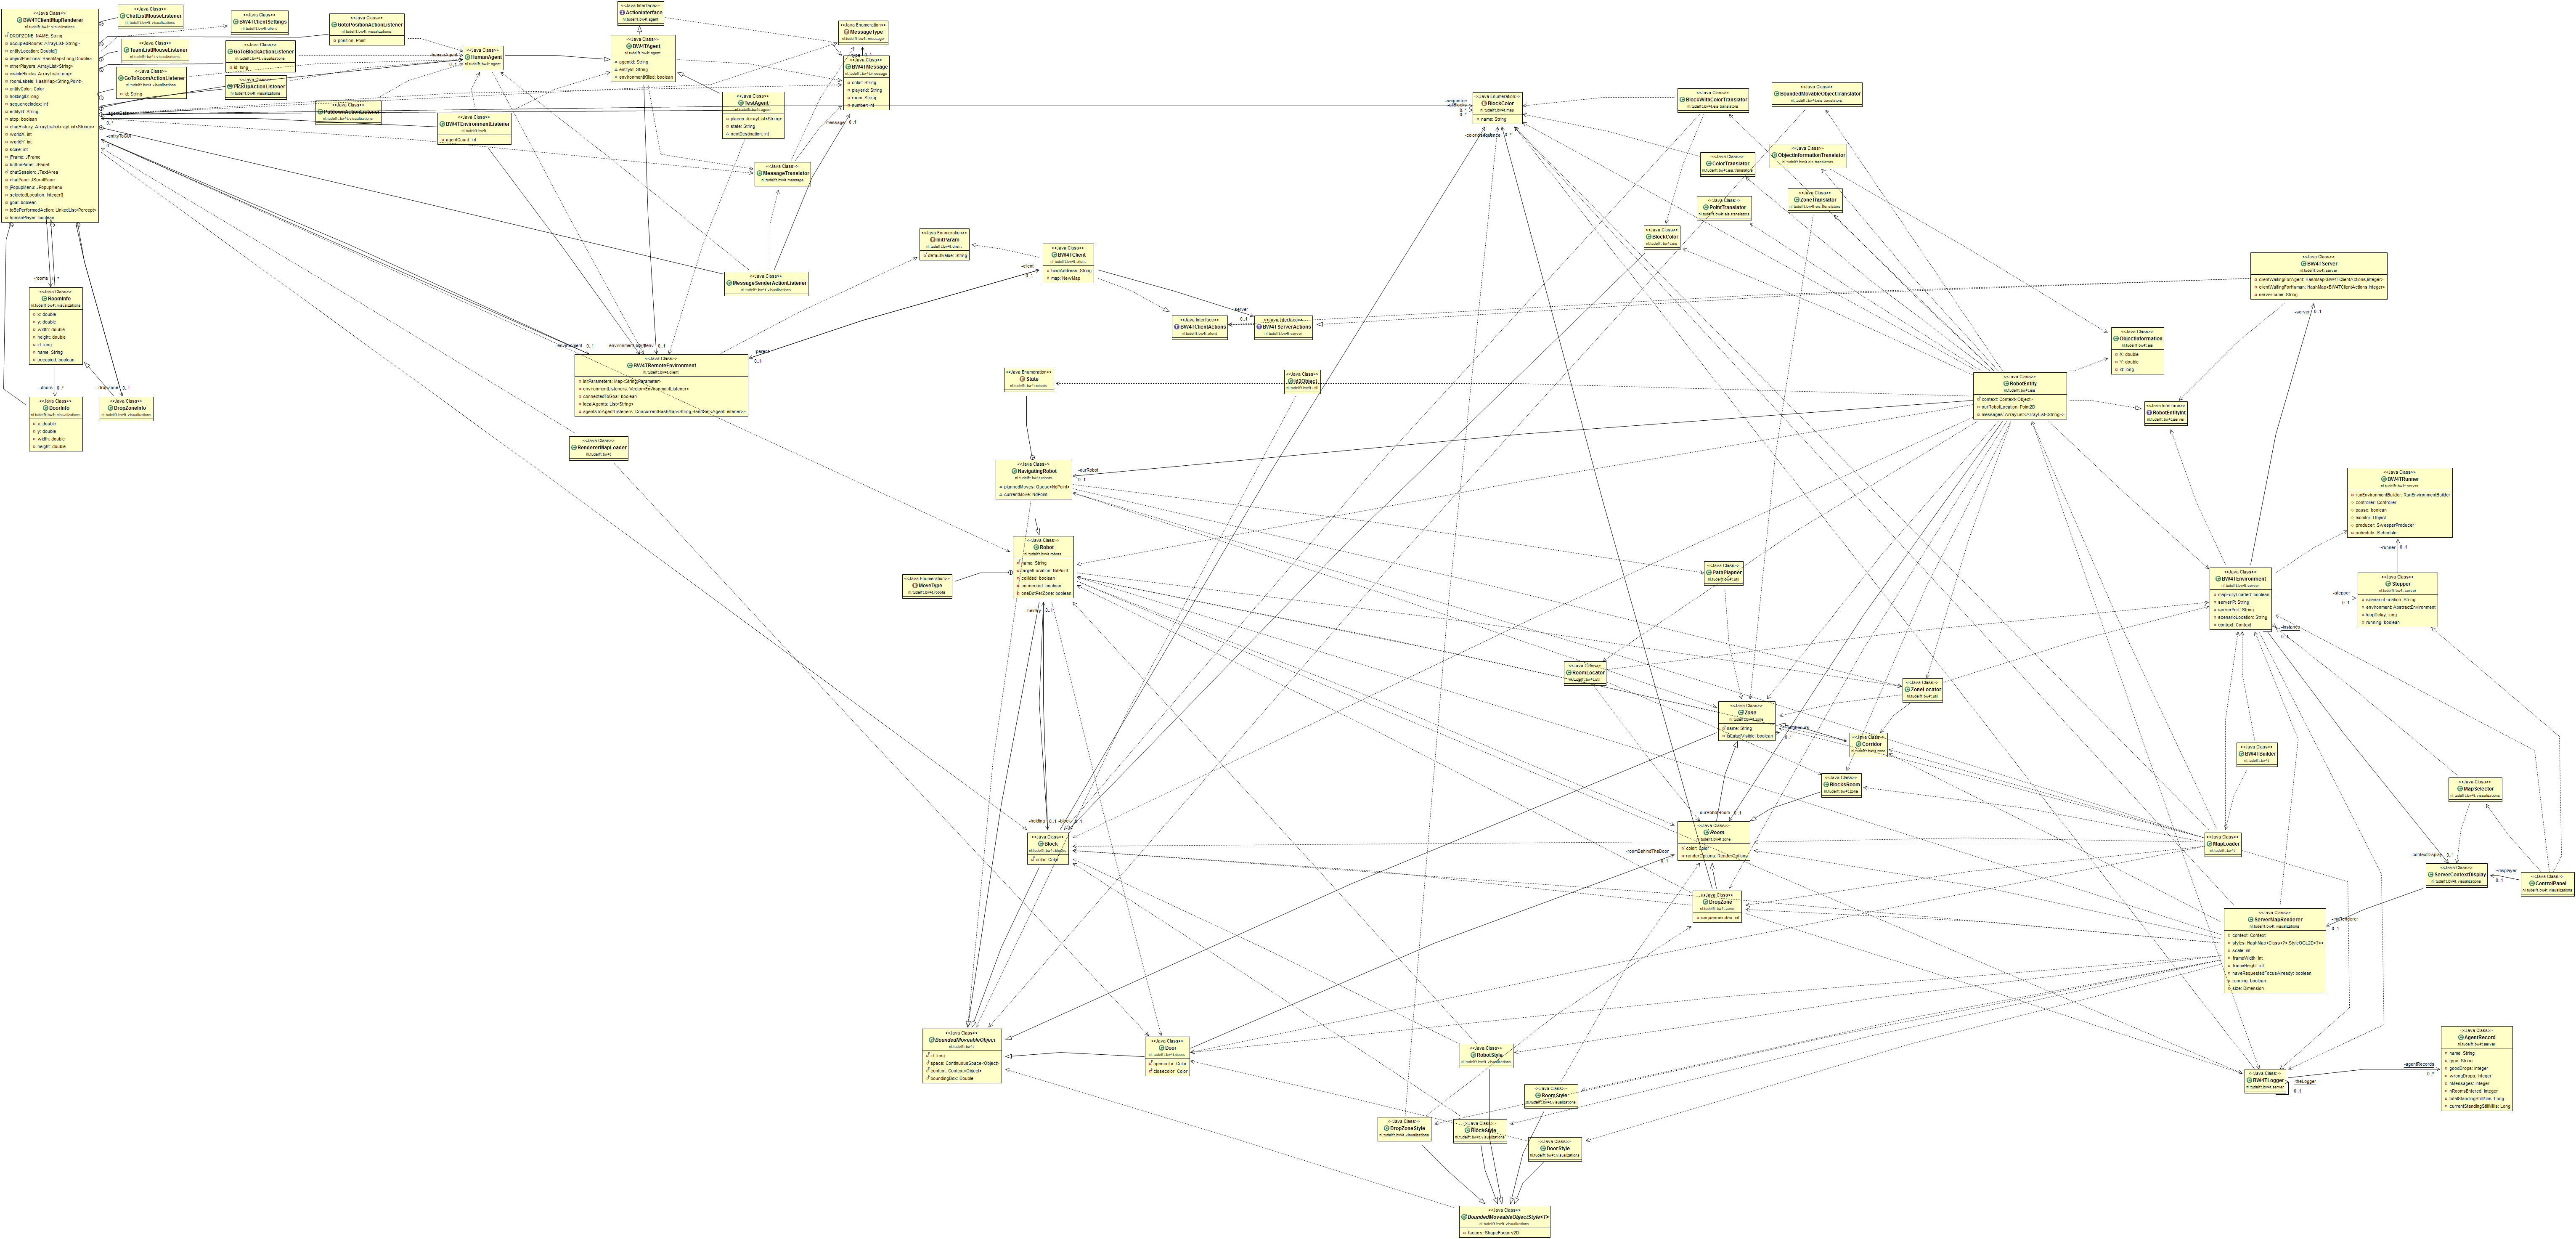
\includegraphics[width=\linewidth]{old.png}
Zoals in het UML diagram te zien is zijn veel klasses met elkaar verbonden. De docmentatie is erg matig en er zijn geen testen. Deze factoren zorgen ervoor dat het heel lastig is om de code te begrijpen en te debuggen. Het is lastig uit te vinden wat een stukje code doet, wat de functie van een methode is, wat het verschil is tussen bepaalde methodes en klassen en wat de connectie is tussen stukken code. \\
In het huidige systeem zit Repast, maar veel functies die ook in Repast zitten worden apart geimplementeerd. Hier zorgt Repast ervoor dat de totale size van de systeem erg groot is (500 mb voor Repast alleen). \\
In het huidige systeem zit een client en server klasse, maar de client en server worden niet consistent gebruikt. De client en server zitten niet los van elkaar, en er zijn klasses die met elkaar communiceren buiten de client en server om terwijl ze dit niet zouden moeten doen bij een client-server architecture. \\
Het opstarten van het systeem is nu ook niet heel gebruiksvriendelijk, de client en server moeten apart opgestart worden. 
Zie ook bijlage voor voorbeelden van 'slechte' code en comments.

\section{Wat hebben we tot nu toe bereikt}
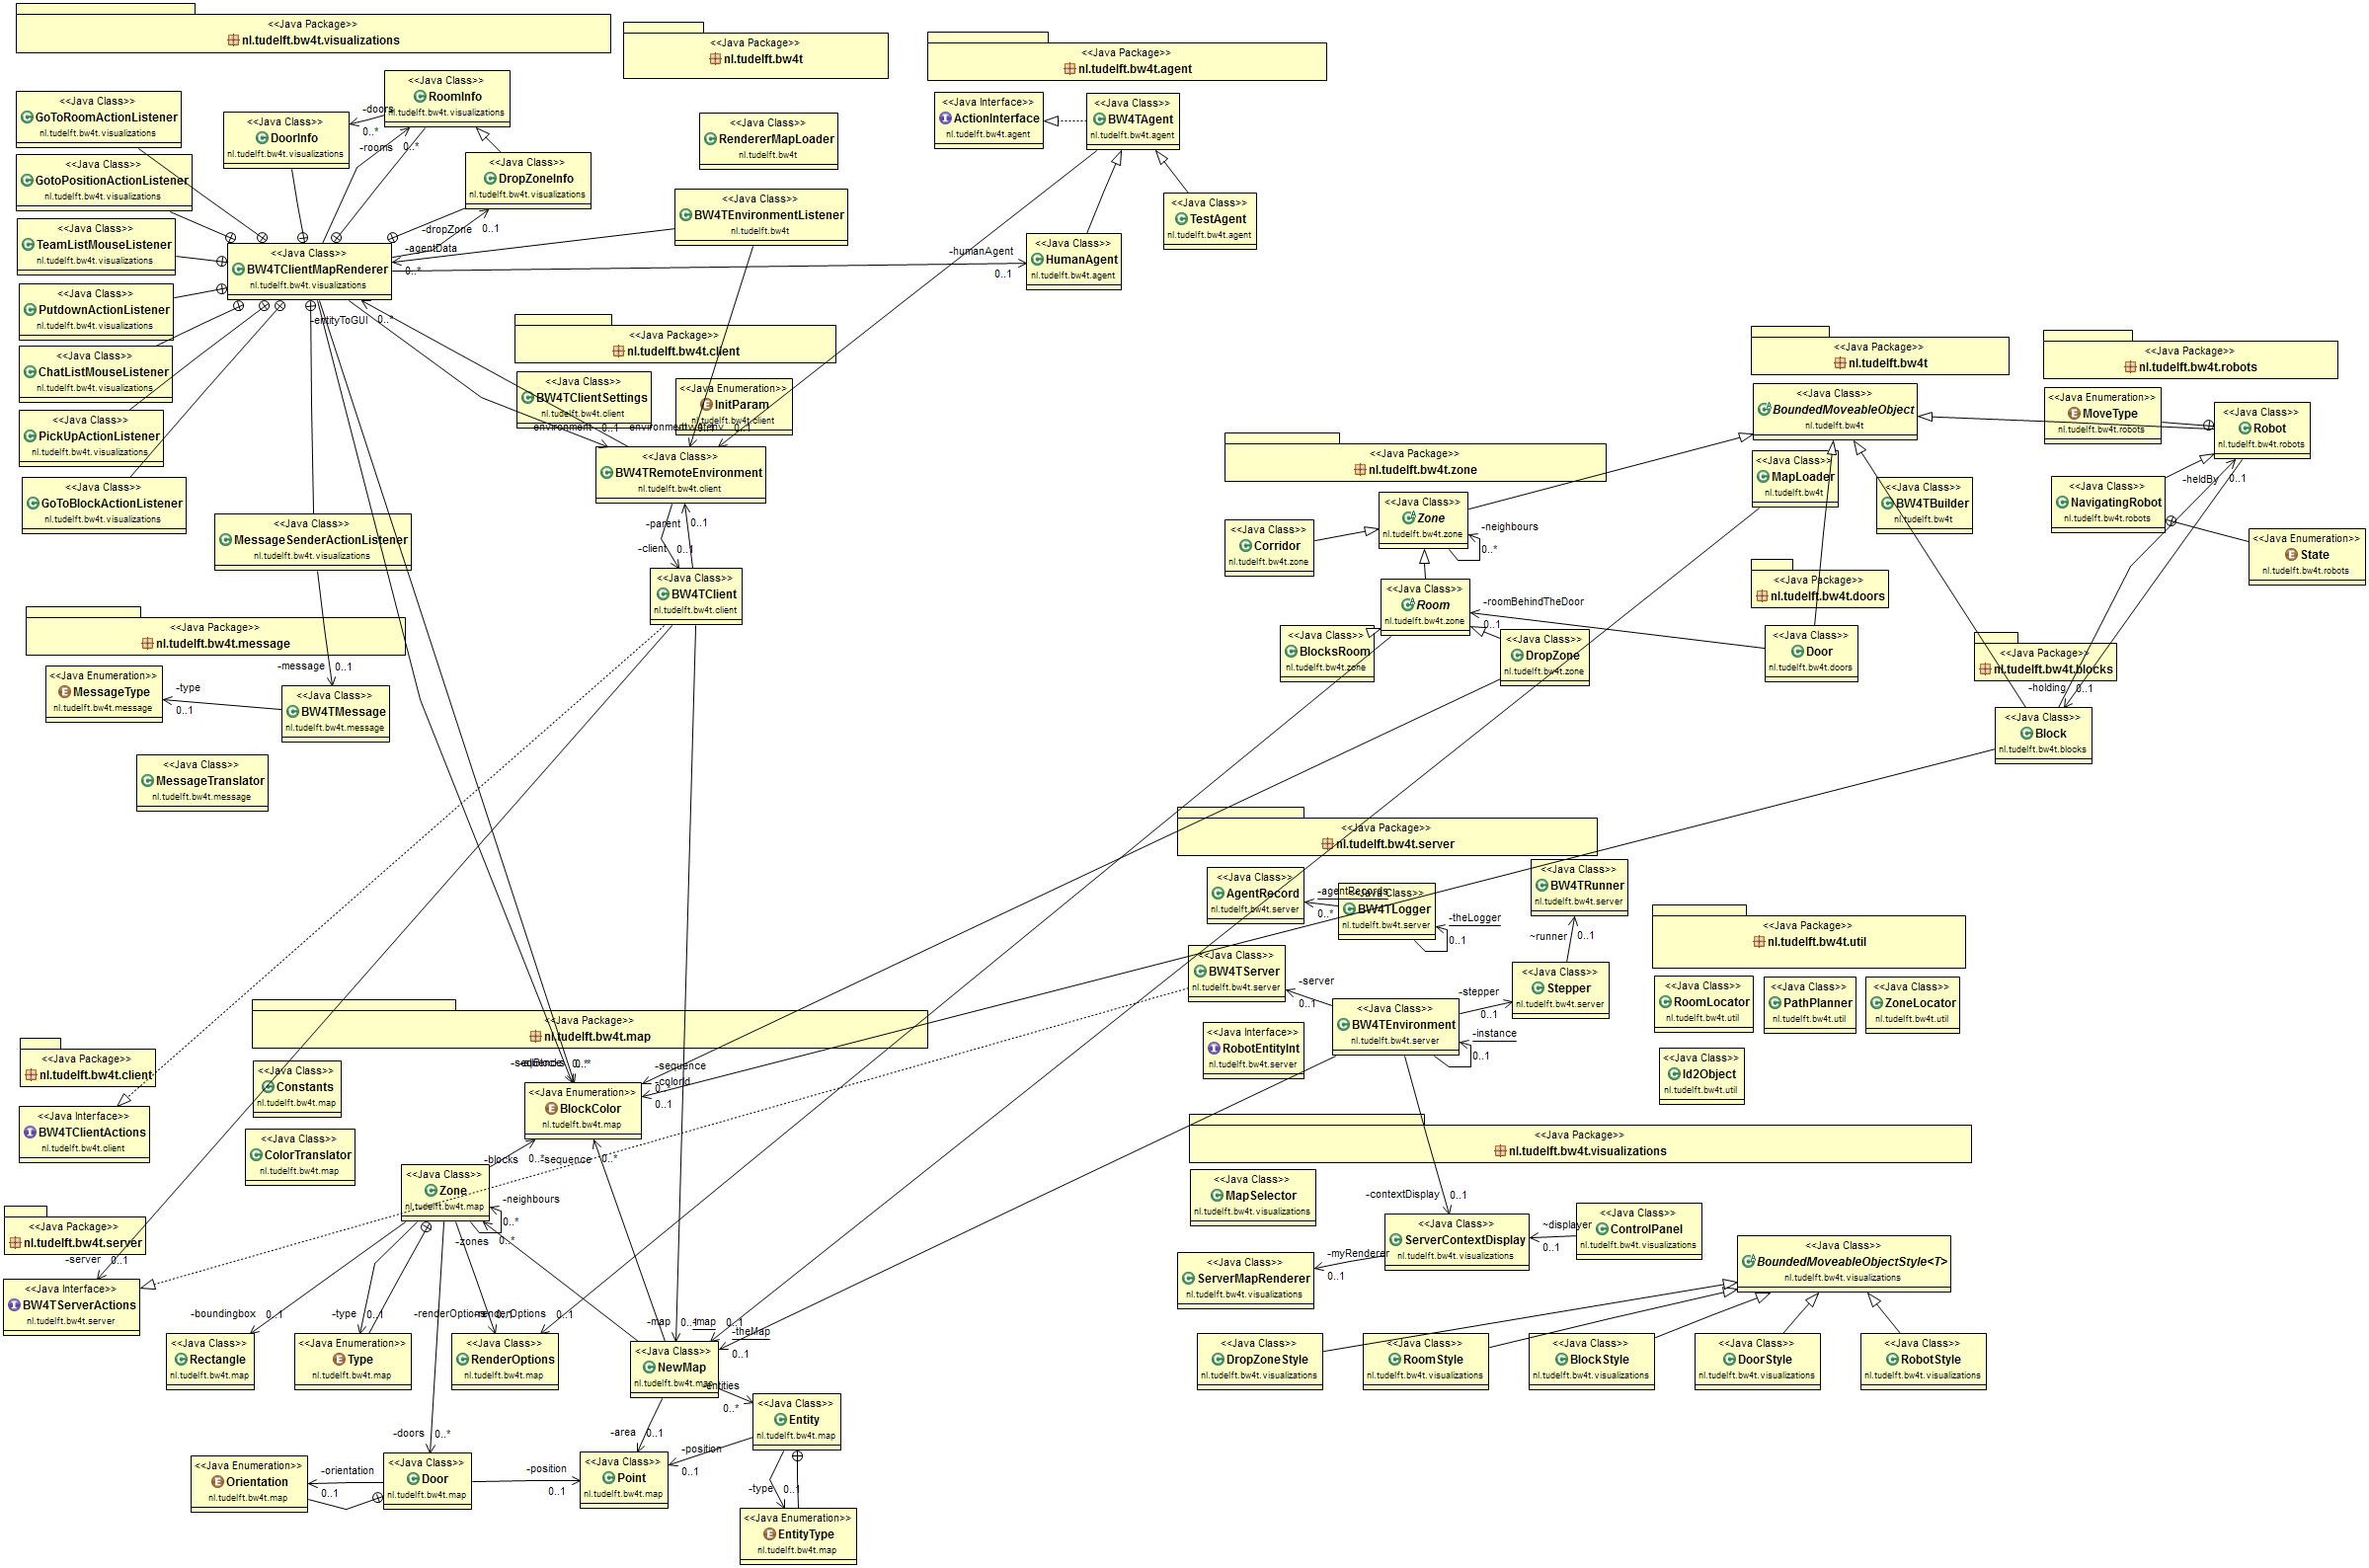
\includegraphics[width=\linewidth]{UMLv2.png}
Repast is nu een plugin en de bijbehrende jar files zijn uit het systeem, wat veel minder ruimte kost (nu nog maar 8mb). De plugin is de nieuwste versie van Repast. \\
We zijn bezig geweest met het splitsen van de server, client en een core. In core zitten de klassen die zowel door de server en de client gebruikt wordt. Elk van deze onderdelen is nu een apart Maven project. Met deze structuur hopen wij meer overzicht te krijgen in de code en dat het voor andere mensen ook (snel) duidelijk is hoe het systeem in elkaar zit. Verder is het testen van het systeem met deze structuur een stuk makkelijker. 

\section{Repast}
Repast is zeker een goed platform voor agent-based modeling. Echter in dit project niet heel nuttig, dit omdat GOAL totaal onafhankelijk werkt van Repast. Het is niet mogelijk om te zorgen dat GOAL en Repast goed synchroon lopen zonder GOAL daarop aan te passen. Wij zijn van mening dat Repast alleen gebruikt kan worden als het systeem helemaal opnieuw wordt opgebouwd en er aanpassingen aan GOAL gemaakt worden. \\
Repast erin laten zitten heeft voor ons op dit moment geen toegevoegde waarde, alles wat Repast biedt moet in dit systeem net anders gebruikt worden. De klasses en methodes moeten dan toch op een eigen manier worden geimplementeerd. Dit geldt ook voor eventuele toekomstig functies van Repast, deze kunnen heel nuttig zijn voor systemen zoals BW4T maar alleen als deze hierop gebouwd zijn.

\section{Wat kunnen wij aankomende weken nog bereiken}
Wat wij de aankomende weken nog kunnen doen is zorgen dat het opstarten van het systeem makkelijker is. Dus dat de server en client niet apart opgestart hoeven te worden, maar dat er een launcher is die alles voor je doet. \\
Ook zullen we de client-server architecture verder uitwerken. Hierbij willen we proberen om het systeem te versimpelen door overbodige connecties tussen klasses te verwijderen of om te zetten naar client-server communicatie. Ook zullen we de documentatie van het systeem proberen te verbeteren. \\
Een ander punt waar we aan gaan werken is het schrijven van testen. Dit zullen voornamelijke functionaliteitstesten zijn. 

\section{Wat zou er kunnen gebeuren}
Als we meer tijd en ervaring zouden hebben zouden we het hele systeem omgooien. Zodanig dat de server-client architecture nog beter wordt geimplementeerd, de documentatie duidelijk is, en alles in het systeem goed getest is. Bij een langerlopend project is het te overwegen om alsnog Repast te gaan gebruiken. Dit zou dus betekenen dat er ook goed naar de link tussen GOAL en Repast gekeken moet worden. \\
Het is dan ook heel belangrijk dat het overzicht bewaart blijft, dat er kritisch naar de code wordt gekeken zodat het systeem optimaal werkt.

\newpage
\textbf{Bijlagen} 
Deze bijlage bevat een aantal voorbeelden van 'slechte' code en comments. Het zijn situaties die we willen verbeteren en voorkomen. \\

Lege methodes \\
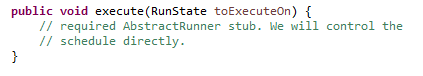
\includegraphics[width=\linewidth]{emptyMethod.png} \\ 

Twee methodes die op elkaar lijken maar niet duidelijk het verschil wordt aangegeven. \\
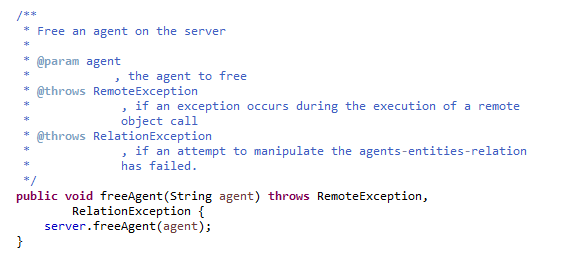
\includegraphics[width=\linewidth]{freeAgentNoClue.png}
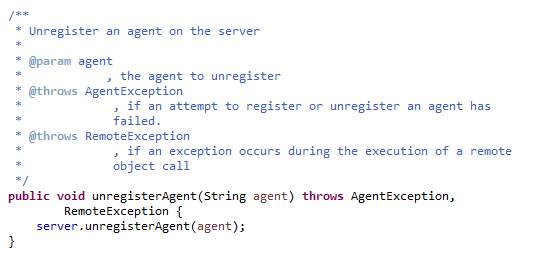
\includegraphics[width=\linewidth]{unregisterAgentNoClue.png} \\ 

Hacks \\
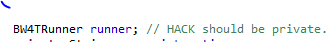
\includegraphics[width=\linewidth]{HackWTF.png} \\ 

Uitgecommende code, zeker bij een eindversie is het netter om dit eruit te halen \\
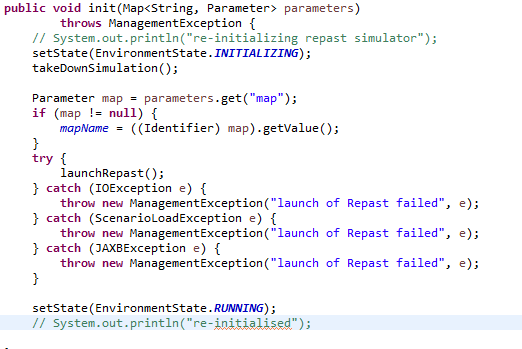
\includegraphics[width=\linewidth]{lelijkCode.png} \\ 

Er wordt niet gechecked of er inderdaad aan de voorwaarde wordt voldaan dat alle entities en agents ontbonden zijn\\
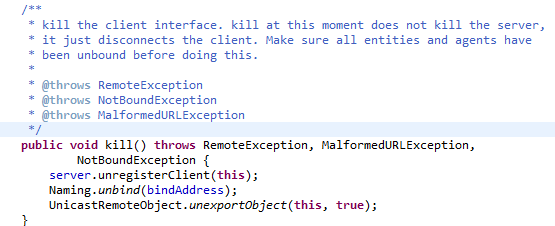
\includegraphics[width=\linewidth]{noEntityCheck.png} \\ 

Niet getest, op de gok iets proberen \\
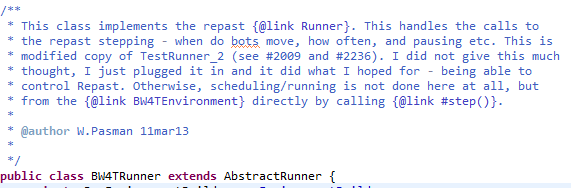
\includegraphics[width=\linewidth]{notTested.png} \\ 

Zou gedaan moeten worden, maar is dus niet gedaan \\
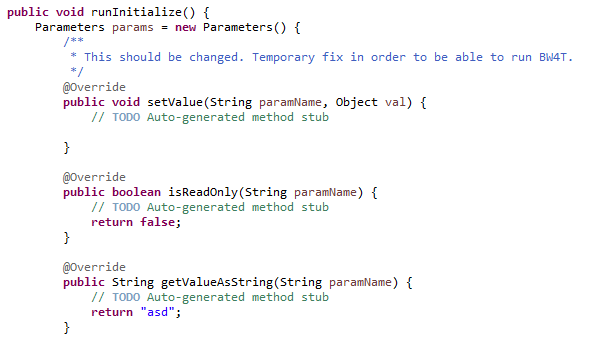
\includegraphics[width=\linewidth]{TODOs+shouldBeFixed} \\

\end{document}
